\documentclass[a4paper,11pt]{report}

\usepackage[a4paper,left=3cm,right=3cm,top=2.5cm,bottom=2.5cm,includeheadfoot]{geometry}
\usepackage[utf8]{inputenc}
\usepackage[english]{babel}
\usepackage{fancyhdr}
\usepackage{amsmath}
\usepackage[noabbrev,capitalise]{cleveref}
\usepackage[square]{natbib}
\usepackage{url}
\usepackage{graphicx}
\usepackage{listings}
\usepackage{chngcntr}
\usepackage{graphicx}
\usepackage{color}

%REMOVE - DARK MODE
%\usepackage{xcolor}
%\pagecolor[rgb]{0,0,0} %black
%\color[rgb]{0.5,0.5,0.5} %grey 

\fancyhf{}
\chead{\leftmark}
\cfoot{\thepage}
\setlength{\headheight}{14pt}
\renewcommand{\headrulewidth}{0.5pt}
\newcommand{\HRule}[1]{\rule{\linewidth}{#1}}

\counterwithout{figure}{chapter}
\counterwithout{table}{chapter}
\counterwithout{equation}{chapter}

\begin{document}

%title page
\title{ 
    \vspace{-4cm}
    \begin{figure}[h]
    \centering
    
\includegraphics[width=0.3\textwidth]{figures/ub_logo.png}
    \end{figure}
    \vspace{1cm}
	\HRule{2pt}\\
	\LARGE \textbf{Exploring the Capabilities of Automatic 3D Model Generation: A Comparative Study}\\
	\HRule{2pt}\\
	\vspace{2cm}
	\normalsize Bachelor's Thesis\\
	\vspace{0.5cm}
	in the applied computer science course of the faculty of business informatics and applied computer science at the Otto-Friedrich-University of Bamberg\\
	\vspace{0.5cm}
	Faculty of Computer Graphics\\
	\vspace{4cm} %4cm is normal, change if title is fixed
}

\date{}

\author{
    \begin{minipage}{\textwidth}
    \begin{flushleft}
    Author: Andreas Franz \textsc{Schwab}\\
    \vspace{0.5cm}
    Examiner: Prof. Dr. Sophie \textsc{Jörg}
    \end{flushleft}
    \end{minipage}
}

\maketitle
\begin{abstract}

The exploration of automatic 3D model generation represents a significant stride in the realm of computer vision and machine learning. This thesis delves into the capabilities of this innovative technology, focusing on a comparative study of various methodologies that facilitate the creation of 3D models from textual and image inputs. The importance of this topic stems from the increasing demand for efficient and accurate 3D model generation in various applications, ranging from virtual reality and gaming to medical imaging.

Despite the advancements in this field, there exists a research gap in comprehensively understanding and comparing different automatic 3D model generation techniques, particularly in the context of their effectiveness, accuracy, and applicability. This thesis aims to bridge this gap by conducting a thorough analysis of selected methods, including Dreamfusion, Fantasia3D, and Magic 3D for text input, and Magic 123 and Wonder3D for image input. The research methods include a detailed experimental setup that uses both subjective evaluations and performance metrics to analyze these technologies.
    
The key message of this thesis highlights the differentiated capabilities and limitations of the individual methods and provides insights into their applicability and potential for future development. The results show significant differences in the accuracy and efficiency of the methods examined and highlight the strengths and weaknesses of the individual techniques in different scenarios.
    
By offering a comprehensive comparison of various methodologies in automatic 3D model generation, this thesis not only aids in the understanding of these technologies but also paves the way for future research, particularly in addressing generative biases and exploring emerging trends.

\end{abstract} 

%toc
\pagenumbering{Roman}
\setcounter{page}{3}
\setcounter{tocdepth}{2}
\tableofcontents


%tables, figures
\listoftables
\listoffigures
\newpage

%content
\pagestyle{fancy}
\pagenumbering{arabic}
\setcounter{page}{1}

\chapter{Introduction}~\label{ch:introduction}

In today's rapidly evolving digital landscape, the demand for 3D models continues to grow, driven by the ever-increasing need for immersive and realistic visual experiences. Generative AI techniques have proven to be a transformative force, enabling researchers and practitioners to develop innovative methods that automate the complicated process of creating 3D models. These remarkable innovations can reshape our digital interactions by enabling advanced simulations, in-depth analysis and captivating visualizations of complex real-world phenomena.

Starting out in 3D synthesis can be a challenging experience, particularly for novices with limited prior knowledge. While directly applying the models outlined in Chapter~\ref{ch:models} may appear straightforward, acquiring a more in-depth understanding of the diverse methodologies and their foundational principles greatly enriches the learning process. This deeper understanding not only improves the practical application of these models, but also enables future advances in the field of automatic 3D model generation.

This thesis provides a comprehensive examination into various models and technologies in automated 3D model generation, offering a detailed analysis of their mechanisms, capabilities, and limitations. The study focuses on evaluating the technologies' effectiveness, emphasizing their proficiency in creating functionally robust and aesthetically appealing 3D models. This research contributes to the fields of computer graphics and artificial intelligence, serving as a valuable resource for novices in automatic 3D model generation and inspiring future researchers.

To provide a foundation for this exploration, a comprehensive examination of the fundamentals of 2D generative AI is undertaken. This includes a comprehensive understanding of key generative models such as Variational Autoencoders (VAEs) \citep{kingmaVAE,rezendeVAE}, Generative Adversarial Networks (GANs) \citep{goodfellowGAN} and Diffusion Models \citep{yangdiffusionSummary,hoDDPMs, sohlDDPM}. Additionally, a brief introduction to Contrastive Language-Image Pre-training (CLIP) \citep{radfordCLIP}, Stable Diffusion \citep{rombachStableDiffusion} and Multilayer Perceptron (MLP) is given. The section concludes with an overview of various forms of 3D representation, including Meshes, Point-clouds, Voxels, Neural Radiance Fields (NeRFs) \citep{mildenhallNERF}, Deep Marching Tetrahedra (DMTets) \citep{shen2021DMTet}, and Instant Neural Graphics Primitives (InstantNGPs) \citep{M_ller_2022}.

This research further evaluates various approaches to generating 3D models based on both images and text input. The methods examined include DreamFusion \citep{pooleDreamfusion}, Magic3D \citep{lin2023magic3d}, Fantasia3D \citep{chen2023fantasia3d}, Magic123 \citep{qian2023magic123} and Wonder3D \citep{long2023wonder3d}. Each method presents unique challenges and opportunities, and their results are thoroughly examined through a comparative study. 

The evaluation involves the application of rigorous performance evaluation metrics covering a spectrum of critical aspects. These metrics include the accuracy of the input and results to ensure that the generated models accurately match the input and maintain the intended properties. Also, the level of detail of these models is examined to assess their ability to capture complicated features and nuances. An important criterion is realism, i.e.~the ability of the generated models to reflect the authenticity of their real-life counterparts. Furthermore, technical aspects such as symmetry and model integrity are also examined to check the structural soundness and coherence of the generated 3D models. This comprehensive analysis leads to an in-depth understanding of the strengths and weaknesses of the individual methods investigated.

In addition, this thesis casts a discerning eye towards the evolving landscape of 3D modeling and highlights emerging trends that have the potential to reshape the field. These trends include innovations such as video-to-3D methods that open innovative dimensions in the creation of three-dimensional scenes. Also, the important topic of inherited biases is discussed, highlighting the need for more in-depth research to ensure the fairness of these methods. By exploring these unexplored areas, the aim is to promote a fairer and more progressive future for the field of 3D modeling.
\chapter{Basics}\label{ch:basics}

The chapter provides the groundwork necessary for the comparative analysis of automatic 3D model generation techniques by introducing the key technologies that drive these methods. It is essential to have a common understanding of the 2D generative models and 3D data representations that form the basis of this field.

The chapter begins by offering a brief overview of the most prevalent text-to-2D generative models, as they play a pivotal role in the process of 3D synthesis. This includes Variational Autoencoders (VAEs) \citep{kingmaVAE,rezendeVAE}, which are fundamental in providing probabilistic frameworks for learning complex data representations. Following this, Generative Adversarial Networks (GANs) \citep{goodfellowGAN} are introduced, emphasizing their unique training mechanics involving both generator and discriminator components. Additionally, the chapter explores the realm of Diffusion Models, with a specific focus on Denoising Diffusion Probabilistic Models (DDPMs) \citep{hoDDPMs,sohlDDPM}, while also touching upon Stochastic Gradient Methods (SGMs) \citep{song2019SGM} and Stochastic Differential Equations (SDEs) \citep{song2020score,song2021maximum}.

\begin{figure}[H]
  \centering
  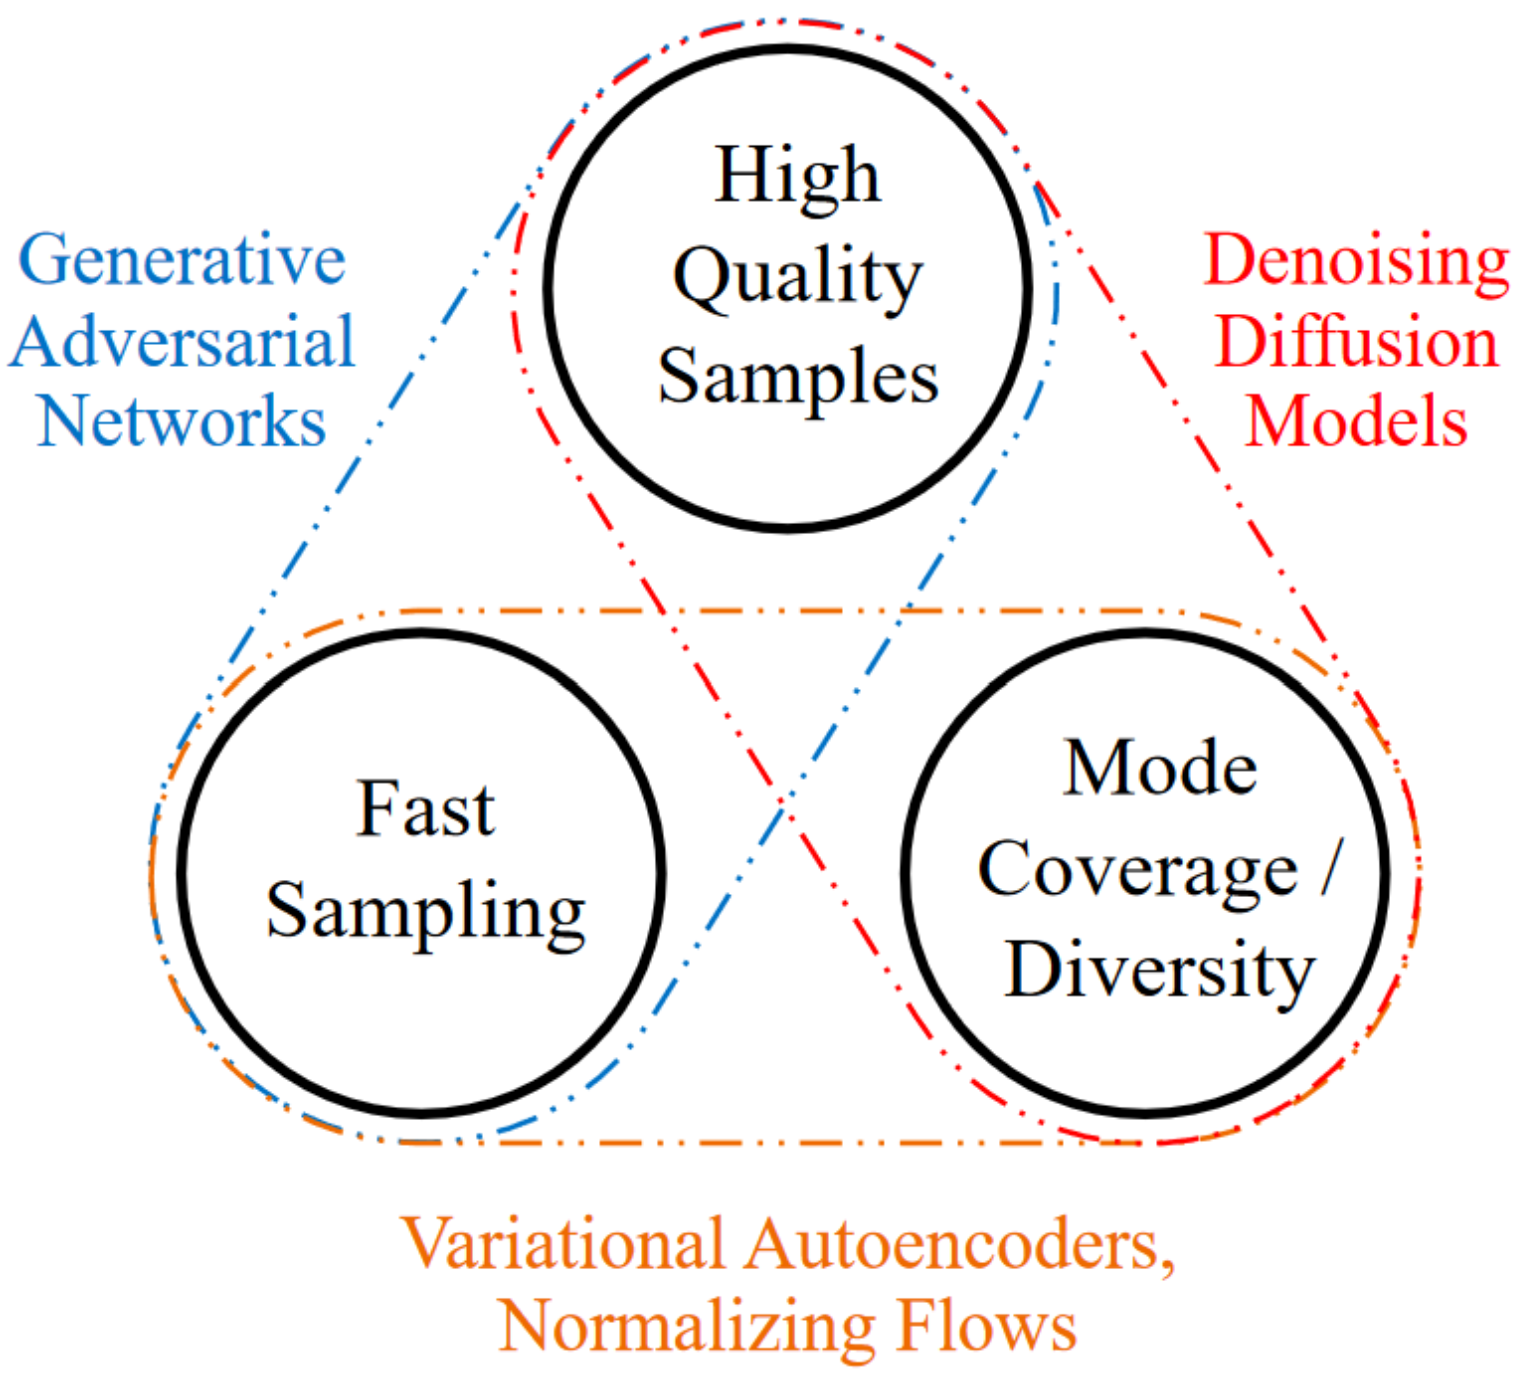
\includegraphics[width=.4\columnwidth]{figures/BasicTrilemma.png}
  \caption{The Generative Learning Trilemma: Balancing Quality, Speed, and Diversity in Generative Models.~\citep{xiao2022tackling}}~\label{fig:generativeTrilemma}
\end{figure}

The figure above from \citeauthor{xiao2022tackling} illustrates the ``generative learning trilemma'', effectively capturing the trade-offs among high-quality sample generation, fast sampling, and mode coverage/diversity in these models. Generative Adversarial Networks are noted for their fast and high-quality samples, Denoising Diffusion Models excel in mode coverage/diversity and sample quality, and Variational Autoencoders balance between fast sampling and diversity in their outputs.

Furthermore, the chapter delves into Contrastive Language-Image Pre-training (CLIP) \citep{radfordCLIP}, illustrating its effectiveness in bridging the gap between natural language and visual data, which is crucial for text-guided 3D model generation. The final part of the chapter is devoted to examining various forms of 3D data representation, such as Meshes, Point-Clouds, and Voxels. Understanding these representations is key to comprehending the structural makeup of 3D objects in computational settings.

//TODO check Final Diffusion Model

\section{Variational Autoencoders - VAEs}
\label{VAEs}

Based on the seminal work by \citeauthor{diggleImplicitPrescribed}, generative models can be classified into two broad categories. Prescribed models employ a well-defined, often parametric, mathematical expression for the probability density function (pdf), which enables easier analytical interpretation of the distributions. In contrast, implicit models synthesize new data samples without relying on an explicit pdf, approximating the underlying data distribution on which they were trained \citep{diggleImplicitPrescribed}. Variational Autoencoders (VAEs), which inherit the foundational architecture of autoencoders, belong to the prescribed models category as they require an explicit formulation of the probability density function (pdf) to function effectively. This feature makes VAEs suitable for tasks that require not only the generation but also the understanding of complex data distributions. \citep{kingmaVAE,rezendeVAE,GoodfellowDeepLearning}. Generative Adversarial Networks (GANs) \citep{goodfellowGAN}, discussed later, are a prime example ofthe latter category.

VAEs are essentially based on the architecture of autoencoders, which consist of an encoder and a decoder. The encoder aims to transform the input data into a low-dimensional latent space representation, commonly referred to as a "code" or "bottleneck" \citep{hintonCode, GoodfellowDeepLearning}. This code captures the most relevant features of the input while reducing its dimensionality. Then, the decoder attempts to reconstruct the original input from the obtained latent vector using a loss function. As explained by Goodfellow et al, an autoencoder that only succeeds in copying the exact representation of the input data does not itself prove useful. The essence of autoencoders lies in their ability to copy approximately rather than perfectly, which forces the model to prioritize which aspects of the input to copy \citep{GoodfellowDeepLearning}. This strategic approach often directs autoencoders to "learns useful properties of the data" \citep{GoodfellowDeepLearning}. To summarize, he main goal of an autoencoder is not the reconstruction itself, but the extraction of a meaningful latent vector that serves as a simplified representation of the input data.

The ability to reduce dimensionality has practical implications for improving the efficiency of classification tasks by reducing computational and memory overhead \citep{GoodfellowDeepLearning}. When paired with information retrieval, this dimensionality reduction makes searching in certain low-dimensional spaces particularly efficient \citep{GoodfellowDeepLearning}. Despite these advantages, traditional autoencoders are not designed to generate new data; their main function is to copy and reconstruct the given input \citep{GoodfellowDeepLearning}.

\begin{figure}[ht]
    \centering
      \hspace{.8cm}
      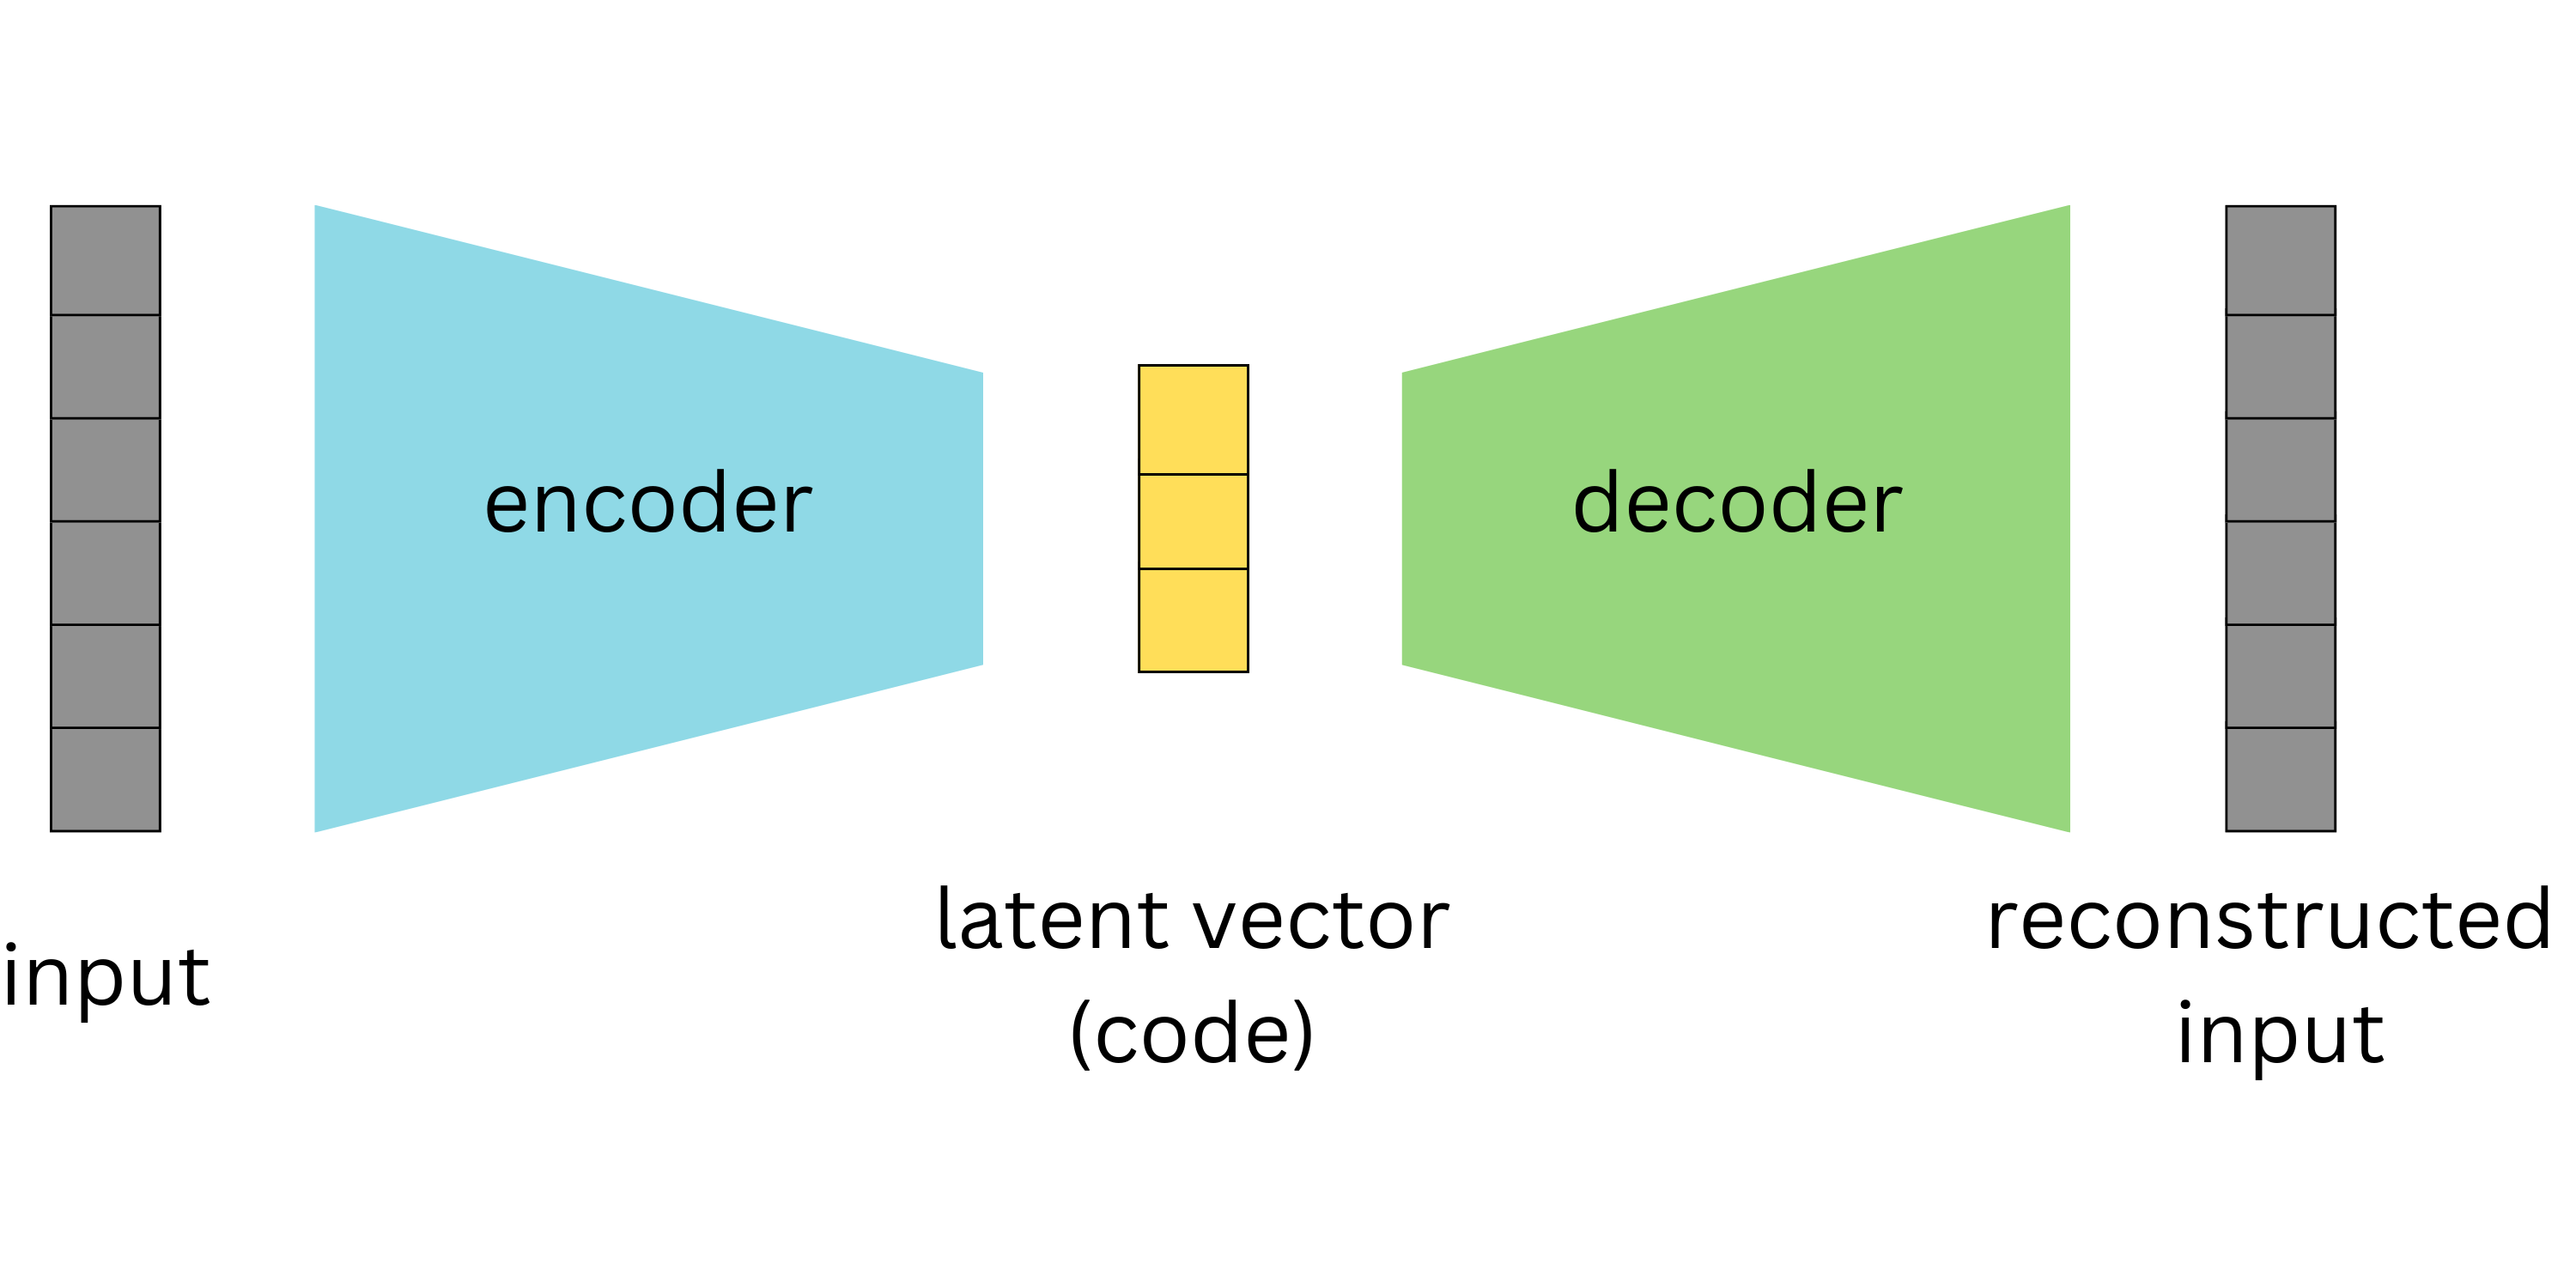
\includegraphics[width=.7\columnwidth]{figures/Autoencoder.png}
      \caption{Autoencoder: The encoder reduces the input dimension to a latent vector that captures the most important features. The decoder then uses this vector to reconstruct the input, with training aimed at minimizing reconstruction loss.}
      \label{fig:figureAE}
    \end{figure}


In variational autoencoders (VAEs), the encoder compresses the input into a space of latent variables and forms a probability distribution over these latent variables called \( q(z|x) \). This distribution helps with robustness against overfitting and enables the model to synthesize new analog data points. During the training phase, VAEs recognize specific regions in the latent variable space, similar to "pools," for different categories of data, allowing for a structured approach to data representation. Unlike standard autoencoders, where it is unclear where a useful latent vector can be sampled for the decoder, VAEs overcome this problem by restricting the latent space to known regions from which vectors can be safely sampled, as cited in \citep{doerschVAE}.

The procedure begins by selecting a sample \( z \) from a code distribution defined by the model, denoted \( p_{model}(z) \). This sample \( z \) is then passed through a differentiable generator network \( g(z) \). A sample \( x \) is then drawn from the distribution \( p_{model}(x; g(z)) \), where its properties are shaped by the processed \( z \) \citep{GoodfellowDeepLearning}. During the training phase, an approximate inference network, also called an encoder \( q(z|x) \), is used to infer \( z \) from \( x \), while \( p_{model}(x|z) \) works as a decoder network to reconstruct \( x \) from \( z \) \citep{GoodfellowDeepLearning}. The main training objective is embodied in the formula:
        
\begin{align}
  L(q) &= \mathbb{E}_{z \sim q(z|x)} \log p_{model}(z, x) + H(q(z|x)) \\
  &= \mathbb{E}_{z \sim q(z|x)} \log p_{model}(x|z) - D_{KL}(q(z|x) || p_{model}(z)) \\
  &\leq \log p_{model}(x)
\end{align}
        
Here, \( L(q) \) acts as a scorecard to evaluate the performance of UAE. The first term \( \log p_{\text{model}}(x|z) \) evaluates how well the UAE can fill in the details to recover the original input, while the second term \( D_{\text{KL}}(q(z|x) || p_{\text{model}}(z)) \) evaluates the complexity of the VAE representation compared to the original term, aiming for simplicity, as mentioned in \citep{GoodfellowDeepLearning}. 
        
The decoder in VAEs either reconstructs the original input or synthesizes new outputs from sampled latent variables. This process is optimized by a loss function that includes both the reconstruction loss and a regularization term based on the Kullback-Leibler (KL) divergence \( D_{\text{KL}} \). This divergence measures the discrepancies between the estimated and true data distributions \citep{kingmaVAE} and improves the model's ability to effectively generalize to unseen data.
        
Through this mechanism, VAEs continuously refine their representation and reconstruction process, improving the generation of new data points that resemble the original training data while maintaining a simplified and structured latent space.

\begin{figure}[ht]
    \centering
      \hspace{.8cm}
      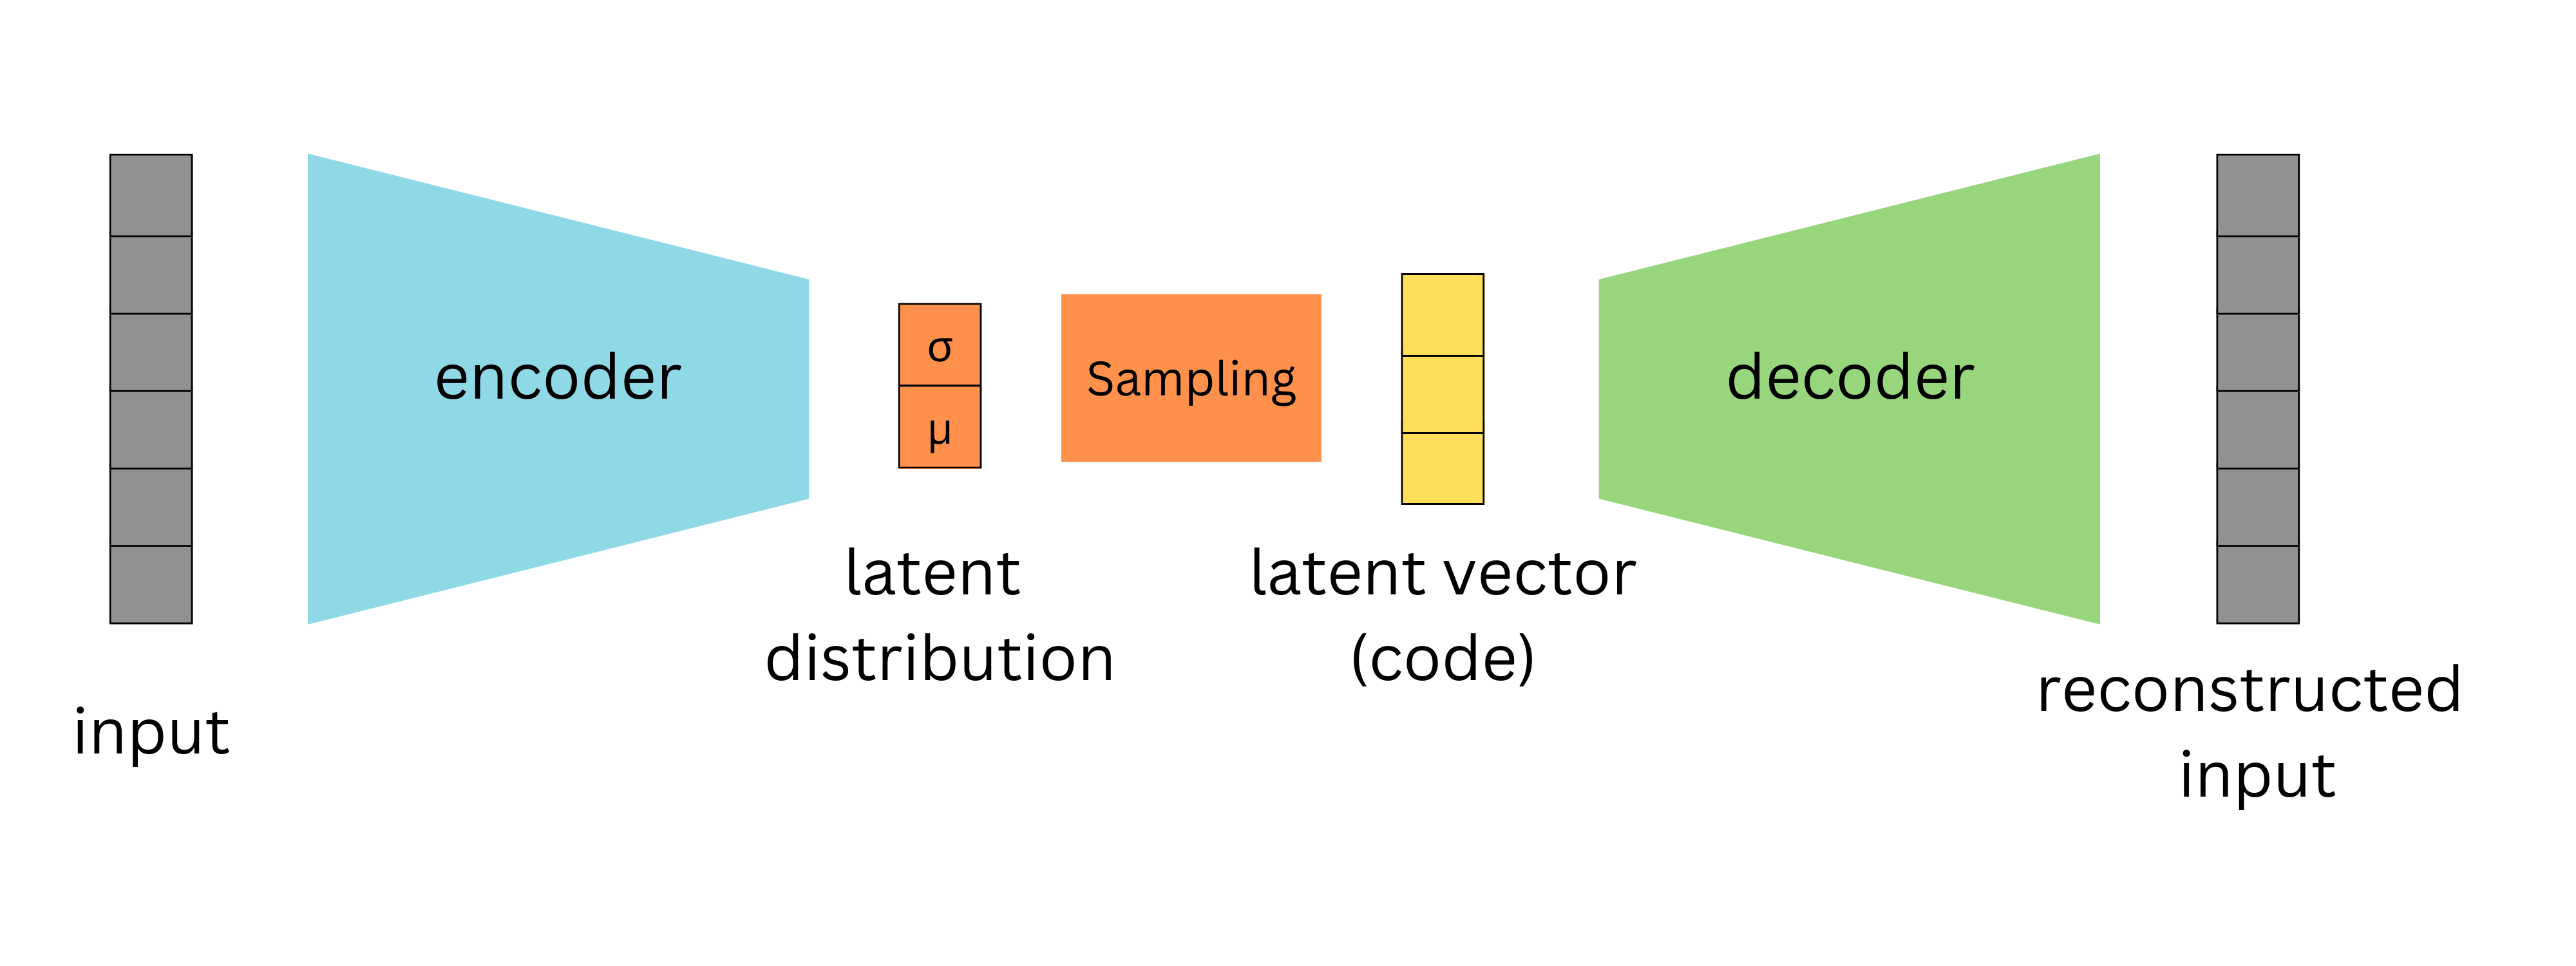
\includegraphics[width=.9\columnwidth]{figures/VAE.png}
      \caption{Functionality of a Variational Autoencoder, demonstrating incorporation of the latent distribution - the mean and standard deviation - for enhancing generative capabilities.}
      \label{fig:figureVAE}
\end{figure}

Despite their capabilities, VAEs exhibit some limitations. According to \citeauthor{GoodfellowDeepLearning}, the generated samples can often be blurry. The reason for this is not fully 
understood, but the blurriness observed may be due to their optimization process, which minimizes Kullback-Leibler divergence. This could lead the model to assign high probabilities to "points that occur in the training set, but may also assign high probability to other points [...] which may include blurry images" \citep{GoodfellowDeepLearning}. The Gaussian distribution often used in VAEs for the generative model may also contribute to this effect, as it can ignore minor features in the input data \citep{GoodfellowDeepLearning}. Another issue is that VAEs typically utilize only a small portion of the latent space, which might further compromise the quality of generated images \citep{GoodfellowDeepLearning}. The performance of the model is also sensitive to the choice of priors for the latent space, making hyperparameter tuning an essential aspect of working with VAEs \citep{kingmaVAE, higginsVAE}. 


\section{Generative Adversarial Networks~--~GANs}\label{GAN}

``When a deep neural network is used to generate data, the corresponding density function may be computationally intractable'' \citep{goodfellowGAN}. Unlike traditional generative models, implicit generative models do not require the explicit design of a density function to describe the patterns in the data. Instead, they use a sample generation process that produces new samples resembling the existing ones \citep{goodfellowGAN}. Before Generative Adversarial Networks were introduced, the leading implicit generative model was the generative stochastic network, ``which is capable of approximately generating samples via an incremental process based on Markov chains'' \citep{goodfellowGAN}. Markov chains are a way of describing a sequence of events or states, where probability of transition to the succeeding state is solely dependent on current states. This approach, however, can be time-intensive and may not always yield accurate results. GANs, on the other hand, directly generate high-quality samples in a single step, bypassing the gradual and often inefficient process of incremental generation.

The unique adversarial nature of GANs arises from the game-like competition between two neural networks: the generator and the discriminator. The generator is responsible for creating fake inputs or samples, which are then passed to the discriminator. The discriminator's role is to differentiate between real samples from the domain set and the fake samples generated by the generator.

\begin{figure}[ht]
\centering
  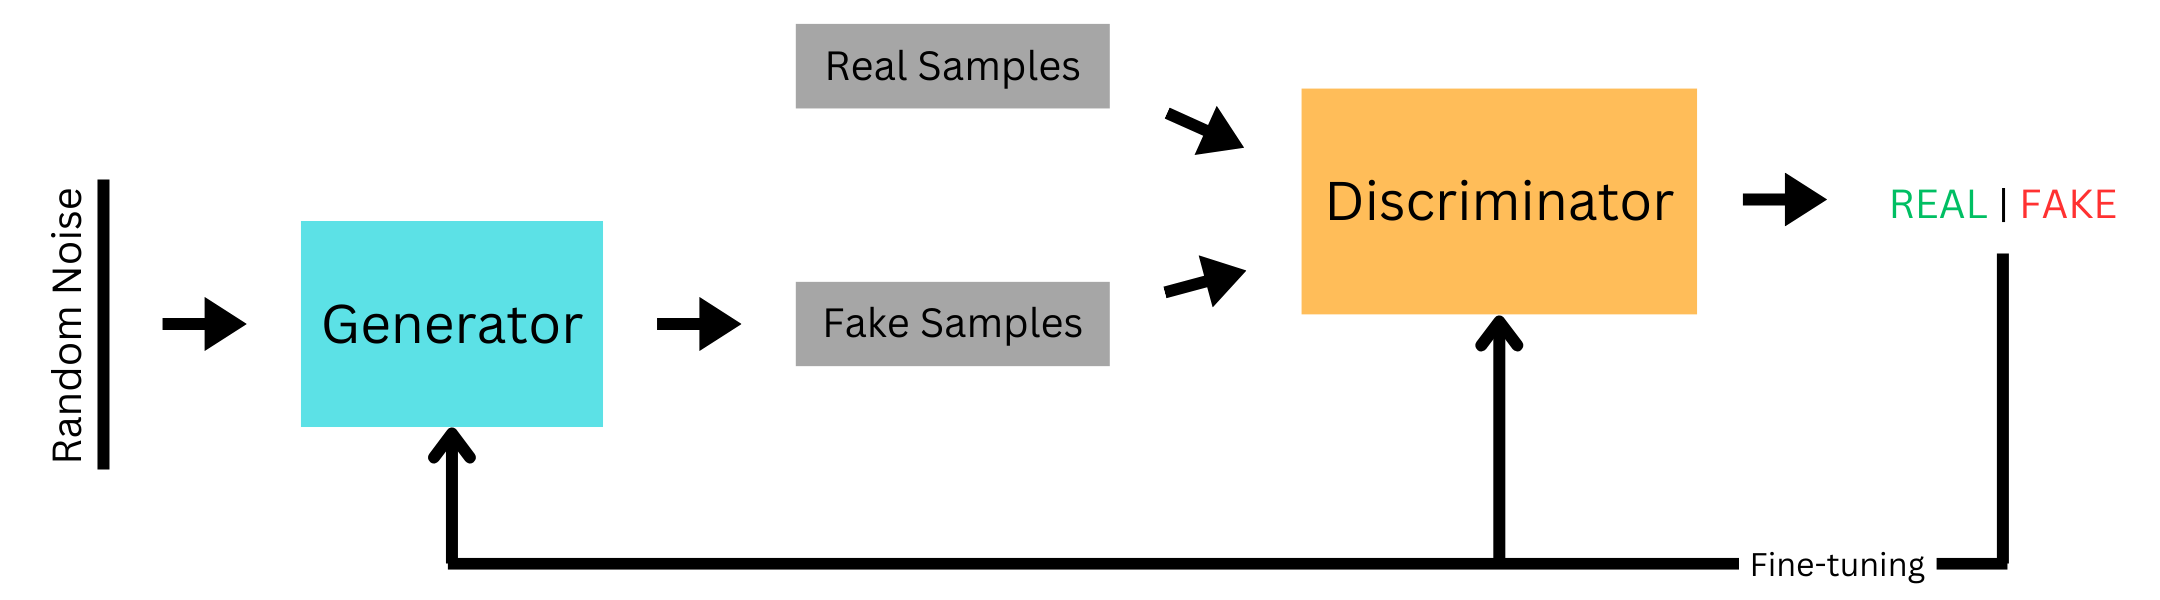
\includegraphics[width=1\columnwidth]{figures/Generator.png}
  \caption{Schematic representation of Generative Adversarial Networks showcasing the interaction between the generator and discriminator networks in generating new data.}\label{fig:figureGAN}
\end{figure}

In the initial training phase, the discriminator is trained on a dataset of real, unlabeled data, learning to identify the characteristics of authentic samples. As the discriminator becomes adept at recognizing all details, the generator starts creating counterfeits, using random input vectors to produce imitations. The discriminator then evaluates these fakes and provides feedback. This feedback loop, involving sample creation and model adjustments, gradually refines the generator's output. Eventually, the generator becomes so proficient that its fakes are indistinguishable from real data, achieving what is known as a zero-sum game, where one network's gain is the other's loss \citep{goodfellowGAN}.

However, the utility of GANs extends far beyond just image generation. Their applications encompass a wide range of fields, demonstrating their versatility and significant impact. These applications include video frame prediction, which is essential in multimedia applications; image enhancement, crucial in improving the quality and clarity of visual data; and encryption, where GANs contribute to the development of advanced security protocols \citep{goodfellowGAN}. One of the most notable features of GANs is their ability to learn in an unsupervised manner, particularly through the generator network. Unlike traditional models that require a supervised learning set with labeled data, GANs can generate new data after training the discriminator with real examples. This capability allows GANs to produce realistic and varied outputs without direct exposure to or reliance on a large labeled dataset \citep{GoodfellowDeepLearning},

% Additionally, GANs play a pivotal role in 3D object generation, the medical field,computer vision as well as traffic control systems, aiding in the development of smarter and more efficient transportation management \citep{AGGARWAL2021100004}.

Nevertheless, GANs pose a substantial challenge in their training process as they are hard to train \citep{goodfellowGAN}. In addition, \citeauthor{brophyGAN} highlight three important problems commonly associated with GANs, among others. These issues, namely non-convergence, diminishing or vanishing gradients, and mode collapse, contribute to the inherent instability experienced during GAN training. Non-convergence refers to the failure of a GAN model to stabilize and reach a state of equilibrium. Instead, it continuously oscillates and fails to converge to a satisfactory solution. As a result, the model does not learn the underlying patterns of the data and can even diverge, leading to poor performance \citep{brophyGAN}. Diminishing or vanishing gradients occur when the gradients used to update the generator become extremely small or even vanish altogether. This phenomenon is often caused by an overly successful discriminator that becomes too adept at distinguishing real and fake samples. As a result, the generator struggles to learn from the feedback provided by the discriminator, impeding its ability to generate high-quality samples \citep{brophyGAN}. Mode collapse happens when the generator collapses, meaning it focuses on producing only a limited set of samples or outputs, typically lacking diversity and variety \citep{salimansNIPS}. In such cases, the generator fails to capture the full range of patterns and characteristics present in the training data, resulting in uniform and repetitive samples that do not adequately represent the true distribution \citep{brophyGAN}.
\section{Diffusion models}
\label{diffusion Models}

The limitations of VAEs and GANs, which were just stated above, have led to the emergence of diffusion models, a method that offer distinct advantages over traditional generative models. Diffusion models operate by progressively perturbing data with noise and then learning to reverse this process to generate new samples. 

~\cite{yangdiffusionSummary} distingueshe between three main approaches that dominate the study of diffusion models, which are going to be discussed shortly: Denoising Diffusion Probabilistic Models (DDPMs) \citep{hoDDPMs,sohlDDPM}, Score-based Generative Models (SGMs) \citep{song2019SGM}, and Stochastic Differential Equations (Score SDEs) \citep{song2020score, song2021maximum}.

\subsection{Denoising Diffusion Probabilistic Models}
DDPMs employ two Markov chains, a forward chain and a reverse chain, also known as the forward and reverse diffusion processes, seen in Figure~\ref{fig:figureForwardProcess} and Figure~\ref{fig:figureReverseProcess} \citep{sohlDDPM}. 

The forward diffusion process is comparable to latent variable models, sharing some similarities with Variational Autoencoders (VAEs), as focus is lying on a latent feature space of the initial data distribution. They differ in the fact that the forward process in DDPMs "is fixed to a Markov chain that gradually [over a span of T steps] adds Gaussian noise to the data according to a variance schedule \(\beta_1, ..., \beta_T \)" \cite{hoDDPMs}. This iterative process continues to add noise "until all structures are lost" \citep{yangdiffusionSummary} resulting in an image of pure noise. The introduction of noise aims to gradually steer the data distribution towards a more manageable prior distribution \citep{yangdiffusionSummary, pooleDreamfusion}. Mathematically, the forward process can be described in two equations:

\[
q(x_t | x_{t-1}) = \mathcal{N}(x_t; \sqrt{1 - \beta_t}x_{t-1}, \beta_t I) \quad \text{where} \quad \sqrt{1 - \beta_t}x_{t-1} = \mu_t \quad \text{and} \quad \beta_t I = \Sigma_t
\] 

\citep{martinez2023understanding}. This describes the process of adding noise to transform a data point \( x_{t-1} \) into a new data point \( x_t \). This transformation is probabilistic and follows a Gaussian distribution \citep{sohlDDPM, hoDDPMs}. The mean value of this distribution is slightly adjusted compared to the previous data point by the factor \( \sqrt{1 - \beta_t} \), which essentially corresponds to the data point \( x_{t-1} \) with a certain noise reduction. The parameter \( \beta_t \) controls the amount of noise added, where a larger \( \beta_t \) means more noise \citep{kingma2023variationalDM}. The covariance matrix, denoted \( \beta_t I \), implies that each element of the data is independently modified with the same amount of noise, since \(I\) represents an identity matrix where all outer diagonal elements are zero \citep{croitoru2023diffusion}.

\[q(x_{1:T} | x_0) = \prod_{t=1}^T q(x_t | x_{t-1}) \] 

\citep{martinez2023understanding}. In the second equation, the focus is on the entire sequence of data points from the original \( x_0 \) to \( x_T \), including all intermediate points \citep{martinez2023understanding}. This expresses the idea that to understand the probability of the entire noisy trajectory, one can calculate the probability of each step from \( x_{t-1} \) to \( x_t \) and then multiply these probabilities together. This is due to the Markov property, which states that each step is only dependent on the immediately preceding step \citep{martinez2023understanding}. This enables a comprehensive view of the transition probabilities over the entire process of noise induction, step by step.

\begin{figure}[ht]
\centering
  \includegraphics[width=1\columnwidth]{figures/manta_DDMP3.png}
  \caption{Forward process adding noise to an image}
  \label{fig:figureForwardProcess}
\end{figure}

The reverse chain is trained to approximate the inverse of the forward process using a deep neural network parameterized with~\(\Theta\), effectively removing the noise added by the forward chain \citep{sohlDDPM, yangdiffusionSummary}. The function \( p_\theta(x_{t-1} | x_t) \) is a probability distribution that estimates how to reverse the diffusion process. Given a data point \( x_t \), it attempts to predict the previous data point \( x_{t-1} \) before noise was added. It is modeled as a normal distribution with a mean \( \mu_\theta(x_t, t) \) and covariance \( \Sigma_\theta(x_t, t) \), both of which are functions parameterized by \( \theta \) \citep{yangdiffusionSummary}.

\[
  p_\theta(x_{t-1} | x_t) = \mathcal{N}(x_{t-1}; \mu_\theta(x_t, t), \Sigma_\theta(x_t, t))
\] 

\[p_\theta(x_{0:T}) = p_\theta(x_{T}) \prod_{t=1}^T p_\theta(x_{t-1} | x_t) \]

\citep{martinez2023understanding}. The latter function \( p_\theta(x_{0:T}) \) represents the probability of the entire sequence of data points from \( x_0 \) through \( x_T \) under the reverse process modeled by the neural network. It starts with an estimate of the final data point \( p_\theta(x_{T}) \) and works backwards through the sequence, multiplying the conditional probabilities \( p_\theta(x_{t-1} | x_t) \) for each step \citep{hoDDPMs,martinez2023understanding}. This function essentially provides a framework for reconstructing the original data from the noisy data by successively removing noise at each step, based on the learned parameters \( \theta \) \citep{yangdiffusionSummary}.


\begin{figure}[ht]
  \centering
    \includegraphics[width=1\columnwidth]{figures/manta_DDMP3.png}
    \caption{Forward process adding noise to an image}
    \label{fig:figureReverseProcess}
\end{figure}


The incremental introduction of the forward and backward diffusion processes offers an advantage as "estimating small perturbations is more tractable than explicitly describing the full distribution with a single, non-analytically-normalizable, potential function" \citep{sohlDDPM}.
According to \citep{hoDDPMs}, the neural network in the reverse process can be trained to predict one of three possibilities: the mean value of the noise at each time step, the original image itself, or the noise of the image \citep{hoDDPMs}. As previously mentioned, the second approach is not as advantageous. Hence, the research focuses on the first and last possibilities, which are essentially identical but parameterized differently. Predicting the image noise allows for straightforward subtraction of the noise from the image, resulting in a less noisy version. By employing this method iteratively, it becomes possible to completely learn an image from noise.

Nevertheless, DDPMs also have their drawbacks with the most severe being the time requirement to generate new samples \citep{xiao2022tackling}. "This is caused by the fact that a Markov process has to be simulated at each generation step, which greatly slows down the process" \citep {martinez2023understanding}. 

\subsection{Score-Based Generative Models}
SGMs are a class of diffusion models that have gained prominence in the field of generative modeling due to their ability to capture complex data distributions and generate diverse and realistic samples.

Score-based generative models (SGMs) take a unique approach to generative modeling by prioritizing the learning of a score function that plays a central role in guiding the generative process. This score function aims to capture the Stein score \citep{steinScore}, which is essentially "the gradient of the log-density function at the input data point" \citep{song2019SGM}. To put it simply, the score can be seen as a vector field, indicating the direction in which the logarithm of the data density experiences the most significant growth \citep{song2019SGM}. In essence, the score function reveals how the data distribution responds to small variations within the data itself, serving as a guiding principle for the generative model. To train a neural network for SGMs, \cite{song2019SGM} employ a technique called score matching \citep{hyvarinenScoreMatching}. This involves estimating the score function for data points intentionally perturbed with Gaussian noise. This means that score matching effectively learns how to denoise the noisy data and restore the original data distribution. \citep{song2020improved}.

In order to generate Samples, Langevin Dynamics \citep{robertsLangevin} is used, which simulates a particle's movement in a field of potential energy, where the score function serves as the guiding force. By moving data samples along the direction of the score function, Langevin Dynamics effectively 'pulls' them toward areas where data density is higher, essentially places where they blend better with the overall dataset.

However, in the specific context of score-based generative modeling, there's a notable challenge to overcome. The estimated score function may not be entirely accurate in regions of the data space where there's minimal or no training data available \citep{song2019SGM}. In such cases, Langevin Dynamics might not converge correctly, resulting in complications during the sample generation process. 

To address this issue, \cite{song2019SGM} suggest "to perturb the data with random Gaussian noise of various magnitudes", while simultaneously estimate the score functions for these noise-altered data distributions. This approach ensures that the resulting data distribution doesn't condense into a lower-dimensional structure \citep{song2019SGM}.






\subsection{Stochastic Differential Equations}
\textcolor{blue}{Score SDEs provide a flexible framework for modeling and generating complex data distributions with inherent stochasticity. Unlike explicit modeling of the joint distribution of data and noise variables, SDEs focus on describing the dynamics of a diffusion process through differential equations. These equations incorporate both deterministic components that govern the overall trend of the process and stochastic components that account for the inherent randomness in the data generation process.
In Score SDEs, the diffusion process is represented as the continuous-time evolution of a random variable. By specifying the drift and diffusion coefficients within the SDEs, one can capture the behavior and evolution of the data distribution over time. The stochastic nature of SDEs allows for modeling intricate dependencies and capturing complex patterns in the data.
Training SDEs involves estimating the parameters of the drift and diffusion coefficients. This is typically done by maximizing the likelihood of the observed data under the SDE framework. Various estimation techniques, such as maximum likelihood estimation or Bayesian inference, can be employed to optimize the parameters.
SDEs can capture long-term dependencies and accurately model the evolution of data over time. Additionally, the stochastic nature of SDEs enables them to generate diverse and realistic samples by incorporating inherent randomness into the data generation process.}

\section{Contrastive Language-Image Pre-training~--~CLIP}\label{CLIP}

\citeauthor{radfordCLIP} address the limitations of traditional computer vision models, which are restricted by their training on a fixed set of object categories and lack adaptability to new tasks or concepts. To overcome these limitations, they propose a novel method called Contrastive Language-Image Pre-training (CLIP), which is an ``efficient and scalable method of learning from natural language supervision''~\citep{radfordCLIP}. This process allows the model to learn a representation of the image that is grounded in natural language, enabling it to understand the content and context of the image.

Unlike traditional computer vision models that rely solely on annotated image datasets, CLIP leverages lots of text and image pairs from the internet. It learns to associate images and their corresponding textual descriptions, allowing it to understand the relationship between visual and textual data. CLIP is built on a transformer-based architecture, which has proven highly effective for natural language processing tasks \citep{radfordCLIP}. It consists of two main components: an image encoder and a language encoder. The image encoder processes images using a modified version of ResNet50 \citep{heResnet} or as a second approach was build upon the Vision Transformer (ViT) \citep{dosovitskiyViT}, while the language encoder uses another modified transformer-based model to process textual descriptions \citep{vaswani2023attention}. By learning to associate images and text, CLIP acquires a generalized understanding of visual concepts and language semantics.

One of the remarkable aspects of CLIP is the ability for zero-shot capability. It can perform tasks without task-specific training \citep{radfordCLIP}. For example, given a natural language prompt, CLIP can recognize objects in images, generate captions, or perform classification tasks.

However, there exist several limitations to CLIP\@. ``The performance of zero-shot CLIP is often just competitive with the supervised baseline of a linear classifier on ResNet-50 features''~\citep{radfordCLIP}.  This means that CLIP is not significantly better than a model that is trained on labeled data for the specific task at hand.
\section{Representation forms of 3D Data}
\label{3Drepresentation}

\subsection{Meshes}
//TODO

\subsection{Point-Clouds}
//TODO

\subsection{Voxels}
//TODO



\chapter{Models}\label{ch:models}

There exist several different approaches to generate 3D Models from a 2D template. In this chapter I will provide detailed insights in some of these approaches. 

\section{3D from Text input}\label{3d from text}

In recent years, the field of 3D model generation has witnessed a significant shift, with an increasing focus on generating 3D models from textual descriptions. This innovative approach leverages advancements in natural language processing and deep learning, allowing for the creation of 3D models based purely on textual input. This section delves into the mechanics and applications of such systems, with a specific emphasis on groundbreaking methods like Dreamfusion, Fantasia3D, and Magic 3D.

The ability to generate 3D models from text opens up a plethora of possibilities. For designers, artists, and architects, it translates to a more intuitive and accessible way to bring ideas to life. This technology also holds immense potential in education and entertainment, where it can be used to create interactive and engaging 3D content. In this section, the focus will be on how these systems interpret textual descriptions while explaining the challenges they face, such as ensuring accuracy and maintaining the fidelity of the generated models to the original text.

%\subsection{Dreamfields}
\label{dreamfields}


(The genesis of DreamFusion lies in the evolution of Dream Fields, a generative 3D AI system unveiled by Google in late 2021. Dream Fields initially married OpenAI's image analysis model, CLIP, with Neural Radiance Fields (NeRF) to foster the generation of 3D views from text. DreamFusion further refined this approach by introducing a new loss based on Google's large AI image model, Imagen, thus paving the way for enhanced text to 3D synthesis.)


Dreamfields present a novel approach to generating three-dimensional objects guided by textual input as introduced by \citeauthor{jainDreamFields}. Utilizing a continuous volumetric representation, Dreamfields are capable of producing high-quality, intricate 3D objects that not only adhere to the specified textual descriptions but also exhibit realistic geometry and appearance. This technology leverages pre-trained image and text encoders, providing a zero-shot learning capability that does not require paired text and object data for training \citep{jainDreamFields}.

The methodology in Dreamfields hinges on learning a continuous volumetric representation, termed a Dream Field, for both the geometry and appearance of a 3D object. The aim is to optimize this Dream Field to be consistent with a given textual description, extending the ideas from previous work on visualizing preferred inputs and features of neural networks by optimizing in image space \citep{jainDreamFields}. The Dream Field is modeled as a neural network, \( f: \mathbb{R}^3 \rightarrow \mathbb{R}^4 \), mapping a 3D coordinate \( (x, y, z) \) toa 4D vector \( (r, g, b, \sigma) \) that represents the color and density at that location. The model then employs raymarching to visualize this continuous field, a computational technique that can be understood as moving a camera through the 3D space to capture the object from various angles. Mathematically, this is achieved by integrating the Dream Field along a ray \( R(t) \) emanating from the camera. Essentially, this is like calculating the average color and light intensity the camera "sees" as it looks along this line. The rendered color \( C \) and opacity, or density, \( \alpha \) are computed using the formulas \citep{jainDreamFields}:

\[
C = \int_0^T \alpha(t) \cdot c(t) \cdot \exp\left(-\int_0^t \alpha(s) \, ds\right) \, dt
\]
\[
\alpha = \int_0^T \alpha(t) \cdot \exp\left(-\int_0^t \alpha(s) \, ds\right) \, dt
\]

Here, \( c(t) \) and \( \alpha(t) \) are the color and density at point \( t \) along the ray, \( T \) is the total length of the ray, and \( \exp \) is the exponential function, used to model how light fades or attenuates as it moves through the object. 

The optimization aims to align the rendered image with a given textual description. This phase focuses on minimizing an objective function \( \mathcal{L} \), which essentially quantifies the difference between the generated object and the textual description \citep{jainDreamFields}.

\[
\mathcal{L} = -\frac{E_{\text{img}}(I) \cdot E_{\text{text}}(T)}{\| E_{\text{img}}(I) \| \, \| E_{\text{text}}(T) \|}
\]

Here, \( E_{\text{img}}(I) \) and \( E_{\text{text}}(T) \) are the embeddings of the image and text, respectively, converted into a common numerical language by pre-trained encoders. \( \mathcal{L} \) is minimized when these embeddings are most similar, measured by the cosine of the angle between them (cosine similarity). In summary, Dreamfields integrates these mathematical principles—continuous mapping through neural networks, raymarching for rendering, and optimization based on similarity measures—to fine-tune the geometry and appearance of a 3D object so that it aligns closely with the given textual description \citep{jainDreamFields}.

Dreamfields find applications in numerous domains where 3D object generation is crucial. These include but are not limited to computer-aided design, virtual reality, and augmented reality. Their zero-shot learning capability opens doors for creating complex objects without the need for extensive training data, making them particularly useful in scenarios where paired text-object data are scarce or unavailable \citep{jainDreamFields}.

Dreamfields' approach to generating 3D objects presents a unique blend of advantages and limitations that contribute to its versatility and potential areas for improvement. Among its most notable advantages is the zero-shot learning capability, allowing the model to generate objects based solely on textual descriptions without the need for paired text-object training data. This attribute is particularly advantageous in scenarios where collecting such paired data is either impractical or resource-intensive \citep{jainDreamFields}. Another significant strength lies in its use of a continuous volumetric representation, which enables the creation of intricate and nuanced geometries. Unlike traditional methods that rely on discrete representations like voxel grids, Dreamfields can generate highly detailed and realistic 3D models \citep{jainDreamFields}. Adding to its merits is the unified treatment of both geometry and appearance in a single representation. Traditional approaches often separate these two aspects, which can result in inconsistencies in the final model \citep{jainDreamFields}. Dreamfields elegantly sidestep this issue, producing 3D objects that are both geometrically and aesthetically coherent. Moreover, the model's optimization process offers a high degree of flexibility, capable of adapting to a wide variety of textual inputs. This makes it a versatile tool for generating a diverse range of objects across different domains. However, Dreamfields is not without its limitations. One of the primary challenges is the computational intensity associated with its continuous representation and optimization process \citep{jainDreamFields}. The high computational requirements could constrain its applicability in real-time or resource-limited settings. Another limitation stems from its reliance on pre-trained text and image encoders, which could introduce biases and restrict the diversity of objects that can be generated \citep{jainDreamFields}. The performance of Dreamfields is significantly influenced by the quality of these pre-trained models, which may vary. Furthermore, the model may struggle with textual descriptions that are inherently ambiguous or open to multiple interpretations. While designed to align closely with textual inputs, the current state of Dreamfields may find it challenging to handle overly vague or abstract descriptions effectively \citep{jainDreamFields}.

Dreamfields offer an innovative approach to 3D object generation through textual guidance. By leveraging a continuous volumetric representation and pre-trained encoders, Dreamfields achieve high-quality, detailed, and realistic 3D objects that closely align with the given textual descriptions. While the technology has its limitations, its advantages and potential applications make it a compelling avenue for future research and development in the field of automatic 3D model generation.


\subsection{Dreamfusion}\label{dreamfusion}

DreamFusion, as introduced by \citeauthor{pooleDreamfusion}, marks a significant advancement in the field of 3D modeling. Utilizing Neural Radiance Fields (NeRF), DreamFusion employs a novel technique known as Score Distillation Sampling (SDS) to generate coherent 3D objects and scenes from a variety of text prompts. This approach diverges from traditional methods that depend on pre-existing images from multiple angles, as DreamFusion dynamically generates these images during training using a diffusion model.

Central to DreamFusion is the use of Differentiable Image Parameterization (DIP), as described by \citep{mordvintsevDIP}. This technique enables the generation of images \( x \) through parameters \( \theta \) and a differentiable generator \( g \), offering refined optimization capabilities even at the pixel level \citep{pooleDreamfusion}. This marks a shift from the conventional approach of diffusion models, which usually produce outputs similar to their training data. In DreamFusion, the parameters \( \theta \) define 3D volumes, with \( g \) functioning as a volumetric renderer. 

In the Score Distillation Sampling (SDS) method, the initial step involves identifying the best parameters \( \theta \) for the model. This involves minimizing the loss in relation to a datapoint created by a model.~\citeauthor{pooleDreamfusion} use the formular~\[ \theta^{*} = \text{arg min}_{\theta} \mathcal{L}_{\text{Diff}}(\phi, \mathbf{x} = g(\theta)) \] This essentially means the model is adjusted to find the parameters \( \theta \) that bring its output as close as possible to the desired result based on textual input. The primary SDS function by \citeauthor{pooleDreamfusion} is:~\[
\nabla_{\theta}\mathcal{L}_{\text{SDS}}(\phi,\mathbf{x}=g(\theta))\triangleq\mathbb{E}_{t,\epsilon}\left[w(t)\left(\hat{\epsilon}_{\phi}({\mathbf{z}}_{t};y,t)-\epsilon\right){\frac{\partial\mathbf{x}}{\partial\theta}}\right]
\] In this equation, \( w(t) \) acts as a weighting factor, modifying the influence of different components within the formula. The term \( \hat{\epsilon}_{\phi}({\mathbf{z}}_{t};y,t) \) represents the score function predicted by the diffusion model \( \phi \). This function estimates the noise adjustments needed based on the noisy image \( z_t \), the text embedding \( y \), and the noise level \( t \). The actual noise at time \( t \) is denoted by \( \epsilon \). This function is key in determining how the noise should be adjusted during the diffusion process to align the generated image with the text input. Additionally, the term \( \frac{\partial\mathbf{x}}{\partial\theta} \) indicates how changes in the model’s parameters \( \theta \) affect the image \( \mathbf{x} \), guiding the optimization process. SDS adds controlled noise to an image \( x \) at each timestep \( t \), and then adjusts it based on the model's scoring, efficiently updating the image to closely match the text descriptions without the need for traditional backpropagation \citep{pooleDreamfusion}.

\begin{figure}[ht]
  \centering
    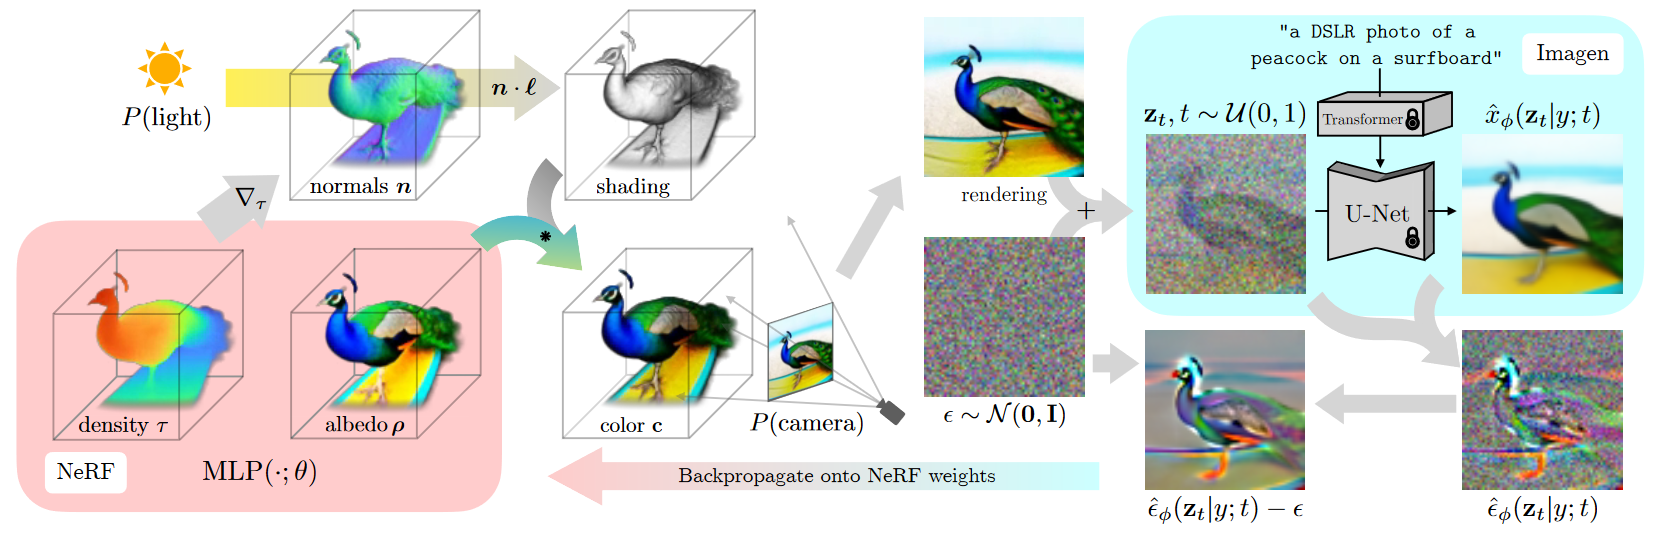
\includegraphics[width=1\columnwidth]{figures/Dreamfusion.png}
    \caption{Summatized functionality of Dreamfusion, image by \citep{pooleDreamfusion}}\label{fig:figureDreamfusion}
  \end{figure}

DreamFusion offers an innovative approach to transforming text into 3D models, as depicted in Figure~\ref{fig:figureDreamfusion}. This process employs several key components: natural language captions for directional guidance, Google's Imagen as the text-to-image diffusion model \citep{saharia2022imagen}, an imporved version of Neural Radiance Field, the mip-NeRF 360 \citep{barron2022mipnerf} ``that reduces aliasing'' \citep{pooleDreamfusion}, and the Score Distillation Sampling (SDS) for the loss function.

At the center of the rendering process is the Neural Radiation Field, which is represented as \( \text{MLP}(\cdot; \theta) \), where the dot \(\cdot\) denotes the input of 3D coordinates and viewing directions. This input is important to determine how light and color interact in 3D space.~\(\theta\) symbolizes the parameters or weights of the MLP that are fine-tuned during training. These parameters determine how the MLP interprets its input (the 3D coordinates and viewing directions) to produce the final output, such as the color and density at each point in the 3D model.

The creation of 3D scenes begins with this parameterization of the NeRF MLP, followed by randomly choosing camera angles and point light positions. This randomness ensures realistic representations from various perspectives. Shading plays a crucial role in adding depth and realism, driven by the interaction of light with surface normals, computed from the density gradients and the light position \( l \). Additionally, the inherent color of objects, or albedo, is generated during the NeRF rendering phase. By combining this albedo with the effects of shading, the NeRF accurately renders the final color for each scene point. The result is a detailed visual representation from the selected viewpoint.

After rendering, DreamFusion evaluates the scene against the diffusion model's predictions, assessing diffusion loss to evaluate the match with the expected outcome. The rendered image is then diffused and reconstructed using a static conditional Imagen model, which adds predicted noise \( \hat{\epsilon}_\phi(z_t | y; t) \) into the rendering, to improve fidelity but also increasing variance \citep{pooleDreamfusion}.

The model refinement phase involves subtracting this predicted noise, resulting in a direction with reduced variance, denoted as \( \text{stopgrad}[\hat{\epsilon}_\phi - \epsilon] \). This direction informs the backpropagation through the rendering process, crucial for updating the NeRF's MLP parameters in a manner that more accurately reflects the scene described by the text. Unlike the SDS method, this backpropagation directly impacts NeRF's rendering pipeline, ensuring parameter adjustments are precisely aligned with the scene's details and nuances.

Despite DreamFusion's promising results, it is not without limitations. The model tends to exhibit a lower level of detail, partly due to its reliance on a \( 64 \times 64 \) image model. Furthermore, while SDS is an effective loss function, it sometimes leads to ``oversaturated and oversmoothed results \([\ldots]\)'' \citep{pooleDreamfusion}. Another aspect to consider with SDS is the mode-seeking behavior, which potentially limits the variety of results generated. This limitation is strengthened by the use of KL divergence, ``which has been previously noted to have mode-seeking properties in the context of variational inference and probability density distilaltion''\citep{pooleDreamfusion}. This tendency of the model to prioritize the most frequent patterns can lead to a trade-off between accuracy and diversity, so ``it may be unclear if minimizing this loss will produce good samples'' \citep{pooleDreamfusion}. This statement highlights a major challenge in machine learning, especially with generative models such as DreamFusion. Minimizing loss, a standard method for improving model performance, does not always lead to high-quality or diverse results. There is a risk of overfitting, where the model can reproduce the training data very well, but is less able to generate new and diverse results.
\subsection{Fantasia3D}\label{fantasia3D}

The model proposed by \citeauthor{chen2023fantasia3d} takes a different approach to generating 3D models from text input, in particular by disentangling geometry and appearance in the generated 3D models.
This method offers a more detailed rendering quality compared to conventional Neural Radiance Fields (NeRFs), which use volume rendering to combine the learning of surface geometry with pixel colors. This conventoional approach limits effective surface recovery, lacking the capability to track the surface of an object and tune detailed material and texture. In contrast, Fantasia3D achieves more realistic outputs with its hybrid scene representation of DMTet, ``which maintains a deformable tetrahedral grid and a differentiable mesh extraction layer; deformation can thus be learned through the layer to explicitly control the shape generation'' \citep{chen2023fantasia3d}

\begin{figure}[ht]
  \centering
    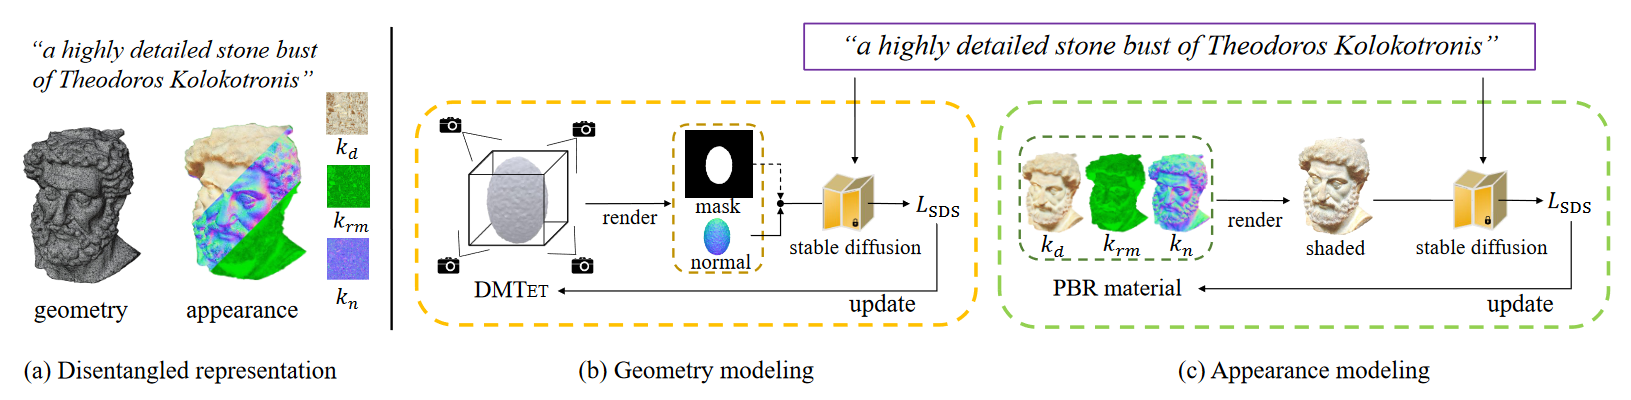
\includegraphics[width=1\columnwidth]{figures/Fantasia3D.png}
    \caption{Overview of Fantasia3D's workflow, disentangling geometry from appearance modeling and iteratively enhancing the quality using a refinment process \citep{chen2023fantasia3d}.}\label{fig:figureFantasia}
\end{figure}

In the geometry stage, Fantasia3D relies on a Deformable Mesh Tetrahedralization (DMTet), which parametrizes the 3D geometry as a Multi-Layer Perceptron (MLP) \(\Psi\). Initially, Fantasia3D renders and encodes surface normals and object masks extracted from DMTet. However, in later stages, the model refines its approach by using only the rendered normal map for shape encoding \citep{chen2023fantasia3d}. The default initialization of DMTet is an ellipsoid, but the model also accepts custom inputs.

Appearance Modeling involves training another MLP \( \Gamma \), which is responsible for applying the Bidirectional Reflectance Distribution Function (BRDF) \citep{chen2023fantasia3d} to a pre-learned DMTet. This function is crucial for ``predict[ing] parameters of surface material and supports high-quality 3D generation via photorealistic rendering'' \citep{chen2023fantasia3d}. The BRDF focuses on the following parameters to achieve accurate shading of the geometry: the diffuse value \(k_d\), the combined roughness and metallic properties \(k_{rm}\), and the normal variation \(k_n\). These are predicted using the formula \((k_d, k_{rm}, k_n) = \Gamma(\beta(p); \gamma)\) by \citeauthor{chen2023fantasia3d}, where \(\beta(p)\) represents the surface properties at point \(p\) and \(\gamma\) denotes network parameters.

Both MLPs (\(\Gamma\) for appearance and \(\Psi\) for geometry) undergo a refinement process, using a pre-trained Stable Diffusion model \citep{rombachStableDiffusion}. This model improves the capabilities of \(\Gamma\) and \(\Psi\), ensuring that they accurately interpret and render 3D shapes and textures. A key aspect of this refinement is the use of Score Distillation Sampling (SDS) loss \citep{mildenhallNERF} for optimization. In this process, SDS loss functions by comparing the true image with the one generated by Fantasia3D. This comparison is achieved through ray casting, where rays are projected for each pixel in the scene. The model then renders the color of each ray, effectively translating the 3D model into a 2D image. This step allows the model to evaluate and adjust its rendering based on how accurately it replicates the true image of Stable Diffusion. By iterating this process, the model continually improves its accuracy in rendering photorealistic images, ensuring that the final output is as close to the actual image as possible.

Fantasia3D offers a high degree of user interactivity, permitting the incorporation of both custom and predefined generic 3D shapes, thus greatly enhancing the versatility and user engagement in the content creation process. The separation of geometry and appearance generation also ensures compatibility with widely-used graphics engines \citep{chen2023fantasia3d}. Despite its capabilities in creating high-quality 3D models from textual descriptions, Fantasia3D encounters specific challenges. One notable limitation is its struggle with accurately generating complex geometries like hair, fur, and grass \citep{chen2023fantasia3d}. Furthermore, the model is currently not able to generate complete scenes as focus is currently lying on individual object generation \citep{chen2023fantasia3d}.

\subsection{Magic3D}\label{magic3D}

Magic3D represents a significant advancement in the domain of high-resolution 3D model generation from text input. Developed by \citeauthor{lin2023magic3d}, this method overcomes limitations observed in previous models like DreamFusion, particularly in terms of optimization speed and resolution of the generated models.

The core technique employed by Magic3D involves a coarse-to-fine optimization process. Initially, a coarse model is generated using a low-resolution diffusion prior, which is then fine-tuned in the second stage to yield a high-quality textured 3D mesh model \citep{lin2023magic3d}. This approach allows Magic3D to generate detailed 3D models with enhanced texture quality in a comparatively shorter time frame.

\begin{figure}[ht]
  \centering
    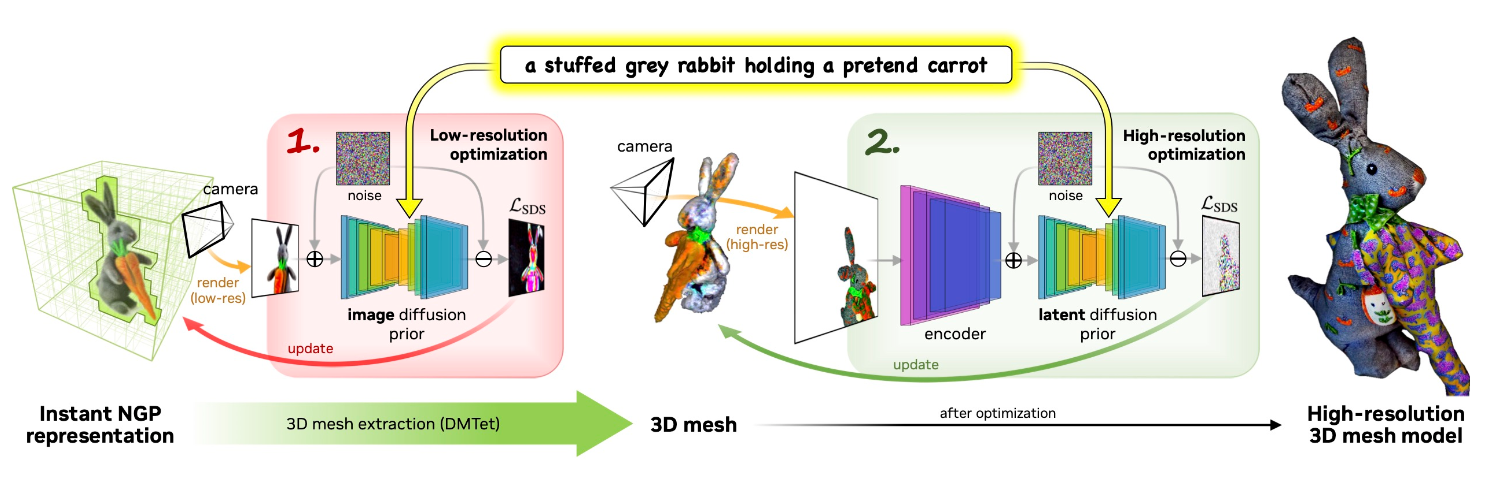
\includegraphics[width=1\columnwidth]{figures/Magic3D.png}
    \caption{This illustration from \citep{lin2023magic3d} showcases the Magic3D process, beginning with the InstantNGP for initial 3D representation. It then details the coarse-to-fine procedure, evolving to a refined high-resolution 3D mesh model.}\label{fig:figureMagic}
\end{figure}


Magic3D's process of generating 3D models from text prompts begins with an initial stage that employs the eDiff-I base diffusion model \citep{balaji2022eDiff-I}, akin to Google's Imagen \citep{saharia2022imagen}. This model operates at a relatively low resolution of \(64 \times 64\), laying the groundwork for the 3D geometry and textures given from the text input \citep{lin2023magic3d}. During this phase, the model uses a sparse 3D hash grid structure from Instant NGP \citep{mueller2022instant}, ``which allows us to represent high-frequency details at a much lower computational cost''~\citep{lin2023magic3d}. The optimization in this phase is performed by two single-layer neural networks that predict albedo (the base color of the object), density (how solid or transparent parts of the object are), and normals (which determine how light bounces off the surface) of the object \citep{lin2023magic3d}. This approach not only speeds up the optimization process but also ensures the foundational quality of the coarse 3D model \citep{lin2023magic3d}. 
This stage involves sampling an image from the NGP representation, which is then infused with an initial state of noise through the image diffusion prior. This step sets the stage for iterative refinement. The refinement is guided by the Score Distillation Sampling (\(L_{SDS}\)) loss function, which evaluates and compares the generated image against a target image, enabling the model to iteratively improve its accuracy. The use of the image diffusion prior in this low-resolution phase is primarily for shaping the overall structure and layout of the model, focusing more on broad features rather than fine details.

In the refinment stage, Magic3D focuses on refining this coarse model into a high-resolution textured mesh, marking a transition from the basic structure to a detailed representation. The refinement process starts with a 3D mesh derived from a deformable tetrahedral grid, where each grid vertex contains a value indicating its distance from the surface (signed distance field) and its deformation from the original position \citep{shen2021DMTet, lin2023magic3d}. The process begins by sampling a new image from this 3D mesh. This image is then processed by an encoder, which converts it into a format suitable for further processing by the latent diffusion model. The latent diffusion model used here, particularly Stable Diffusion \citep{rombachStableDiffusion}, operates at a high resolution of \(512 \times 512\), allowing for more detail of the final model \citep{lin2023magic3d}. Once the latent diffusion prior has processed the image, its output is evaluated using the Score Distillation Sampling \(L_{SDS}\) loss function. This function compares the generated image with a target image, enabling the model to fine-tune each vertex's signed distance field and deformation \citep{lin2023magic3d}. A technique employed here is the increase in focal length to zoom in on object details, essential for recovering high-frequency details in both geometry and texture \citep{lin2023magic3d}. Finally, the mesh is extracted using a differentiable marching tetrahedra algorithm, essential for achieving fine texturing \citep{lin2023magic3d}.

Magic3D's proficiency is not limited to just creating high-quality 3D models; it also offers extensive creative control over the generation process. The model supports ``fine-tuning a learned coarse model with a new prompt'' \citep{lin2023magic3d}, allowing users to influence the generated output significantly. This includes text-based edits and image-conditioned generation, increasing the scope for creative and personalized 3D model generation \citep{lin2023magic3d}.

\section{3D from Image}\label{3d from image}

Converting two-dimensional images into three-dimensional models is a challenge in the field of computer vision and 3D modeling. This section examines some of the methods used in converting 2D images into 3D models. This process has profound implications for various fields, including virtual reality, gaming and medical imaging. Techniques such as Magic 123 and Wonder3D are analyzed to demonstrate some core concepts.

\subsection{Magic 123}\label{Magic123}

//TODO

\begin{figure}[h]
    \centering
      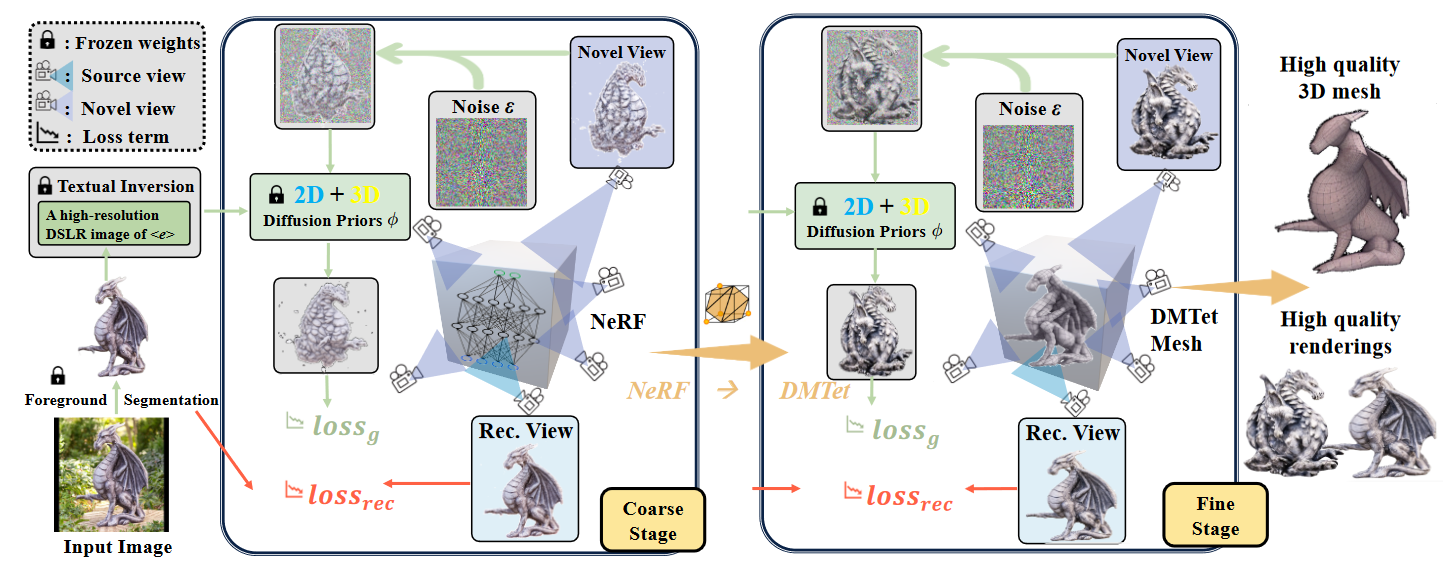
\includegraphics[width=1\columnwidth]{figures/Magic123.png}
      \caption{Summatized functionality of Magic123}\label{fig:figureMagic123}
\end{figure}
\subsection{Wonder 3D}\label{Wonder3D}

The primary innovation of Wonder3D lies in its ability to efficiently generate high-fidelity textured meshes from single images, a task that presents considerable challenges in the field of computer vision.

The method begins by generating consistent multi-view normal maps alongside corresponding color images through a cross-domain diffusion model. This process is critical for ensuring the fidelity and consistency of the generated 3D models. To achieve this, Wonder3D employs a multi-view cross-domain attention mechanism, which facilitates the exchange of information across different views and modalities, thereby enhancing the consistency and quality of the generated images \citep{long2023wonder3d}.

\begin{figure}[ht]
  \centering
    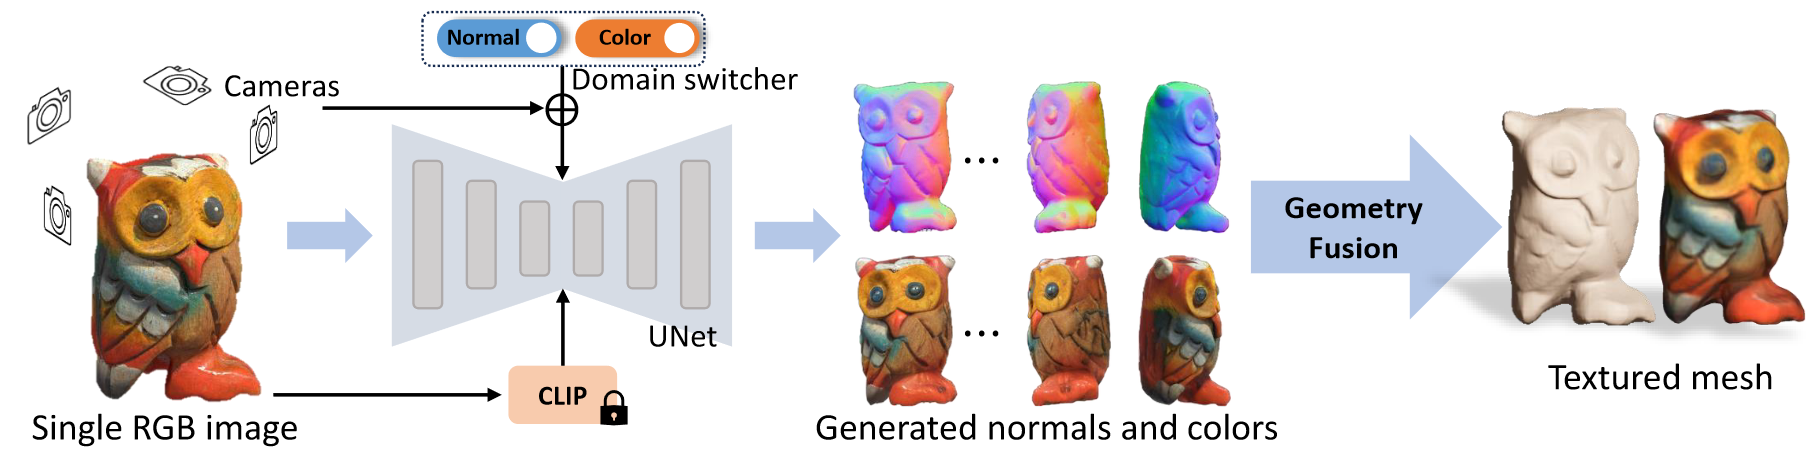
\includegraphics[width=1\columnwidth]{figures/Wonder3D.png}
    \caption{Summarized functionality of Wonder3D, depicting the method's unique approach to generating high-fidelity textured meshes from single images using cross-domain diffusion models \citep{long2023wonder3d}.}\label{fig:Wonder3D}
\end{figure}

An integral part of Wonder3D is its novel geometry-aware normal fusion algorithm. This algorithm robustly extracts high-quality surfaces from the generated multi-view 2D representations, including normal maps and color images. The fusion algorithm plays a pivotal role in reconstructing clean and detailed geometries from these 2D inputs, which is a significant step forward in the field \citep{long2023wonder3d}.

To understand this in simpler terms, imagine you have a single photo of an object, and you want to create a detailed 3D model of it. Traditional methods might struggle with this task, especially in terms of generating a model that is consistent and detailed from all angles. Wonder3D addresses this challenge by first creating multiple views of the object, as if you were looking at it from different angles. It does this by generating normal maps, which are like detailed blueprints of the object's surface textures and contours, as well as color images that match these maps. Then, using its specialized fusion algorithm, Wonder3D combines all these different views into a single, cohesive 3D model. This model not only looks good from the original angle of the photo but also from other angles, making it a more complete and accurate representation of the object.
%\section{3D from Video}
%\label{3d from video}
%//TODO

%\subsection{NERfs}
%\label{nerfs}
%//TODO
\chapter{Comparative Study}
\label{ch:comparative study}

\subsection{Experimental Setup}
details about data collection, preprocessing, and model training

\subsection{Performance Metrics}
discussion of evaluation criteria used in the comparative study

\subsection{Results and Analysis}
present findings and their interpretation


\chapter{Future Directions}
\label{ch:future}
The exploration of automatic 3D model generation has revealed a dynamic and rapidly evolving field. While this thesis has covered several significant models, it's important to acknowledge that these represent just a fraction of the ongoing advancements. The beauty of this field lies in its cumulative progress, where each new model not only builds upon existing knowledge but also introduces innovative approaches to enhance the state-of-the-art. This chapter will highlight some of the most promising research trends and potential directions for future exploration, focusing on both computational efficiency and quality enhancement.

The realm of 3D model generation is marked by continuous advancements, with new findings emerging on a near-weekly basis. Although keeping pace with these developments is challenging, certain areas within this domain warrant ongoing attention and improvement. This chapter will also speculate on future possibilities, acknowledging the dynamic nature of this field where today's cutting-edge advancements may soon become tomorrow's standard practices.


\section{Emerging Trends in 3D Model Generation}
explore current developments and new directions in the field.
Gaussian Splatting
Lumia AI - Genie


Virtual production is becoming increasingly popular, allowing for more creative and cost-effective backdrops. This rise in demand is expected to continue, driving growth in the market for production-ready 3D assets. The concept of the metaverse is also gaining traction, with significant investments from major companies. This virtual environment is set to redefine experiences ranging from virtual concerts to digital clothing, opening new avenues for 3D modeling applications.

Another emerging trend is the standardization of universal modeling standards. As 3D assets are required to function across various virtual platforms, the need for standardization becomes crucial. Tools like TurboSquid's StemCell are paving the way for more versatile and universally compatible 3D models.

Overall, these trends indicate a shift towards more integrated, AI-driven, and standardized approaches in 3D model generation, pointing towards a future where 3D modeling is more accessible, versatile, and deeply ingrained in various aspects of digital interaction.



\section{Potential Research Directions}
suggest areas for future research based on study's findings.
Reduce Computational cost

The future of 3D modeling and additive manufacturing (AM) holds substantial potential for innovation across various sectors. One key area of research is exploring the use of AI in additive manufacturing. With technologies like ChatGPT and Nvidia's AI tools demonstrating the ability to create 3D models from text input, there's a significant opportunity for AI applications to become more prevalent in additive manufacturing.

The healthcare industry is increasingly adopting AM to deliver personalized healthcare solutions. This includes the creation of patient-specific implants and surgical tools customized to individual anatomies. The integration of AM in healthcare facilities for various applications, such as orthopedics, dental, and surgical instrumentation, offers an exciting avenue for research, potentially revolutionizing patient care and treatment.

In industrial markets, the use of metal AM for the production of end-use parts, especially in the aerospace and energy sectors, is experiencing rapid growth. Researching new AM solutions specifically designed for mass production, which combine various printing and finishing technologies, could significantly enhance manufacturing workflows and output

Bioprinting is another promising field, with significant strides being made in using bioprinted human tissue models for drug discovery and development. Researching the ability to simulate human responses to drugs in a laboratory setting using bioprinted models could dramatically streamline drug development processes and potentially eliminate the need for animal testing.

Moreover, there are opportunities to address challenges such as intellectual property protection, managing the complexity of large-scale 3D models, and overcoming adoption barriers due to advanced 3D modeling tools and techniques. These challenges present potential research directions that could significantly impact the field's growth and adoption.

\chapter{Conclusion}~\label{ch:conclusion}
//TODO

\section{Summary of Findings}

This thesis has explored various methods used for automatic 3D model generation, focusing on DreamFusion, Magic3D, Fantasia3D, Magic123, and Wonder3D. Each method was not only introduced but also scrutinized through a comparative analysis. The examination revealed that DreamFusion, one of the earlier methods, tended to produce more blurred outputs compared to its successors. This could be attributed to the initial stages of development in this field. In contrast, newer models like Fantasia3D showed improvements, especially when initiated from a shape approximating the target object. Interestingly, a random sphere as a starting point was found ineffective.

A significant aspect noted was the evolution in speed and efficiency of model generation. Earlier methods required more time for results that aligned with the text prompts, whereas newer models showcased rapid generation capabilities. Despite advancements, challenges in generating intricate details, such as plants, persisted across all methods, highlighting areas for future optimization. Fantasia3D, with its advanced texture generation stage, excelled in producing realistic textures, though it struggled in overall model generation.

One of the most promising developments observed was in the newest methods, such as Genie, which demonstrated fast and detailed outputs, signaling rapid progress in the field. However, the presence of bias in generative AI was a recurring concern, underscoring the need for continued research and development to address this issue.



In a series of tasks testing the capabilities of various 3D rendering methods, distinct patterns emerged across different prompts. For the Playmobil figure, characterized by its uniform base structure, DreamFusion struggled with intricate geometry but maintained color accuracy, while Magic3D excelled in realistic textures and geometric precision for simpler, flat structures. Fantasta3D often overemphasized realism at the expense of essential prompt features, and Magic123, although capturing the essence well, added superfluous elements. Wonder3D frequently failed in even basic details. In the bread prompt, emphasizing symmetry and specific properties, DreamFusion continued to falter with structure, Magic3D showed robustness to directive prompts, and Fantasia3D was disoriented by specificity. Magic123's replication of the input image raised questions about its adaptability, and Wonder3D struggled with overall structure.

When rendering a sleeping dog, a task focusing on organic forms, texture, and anatomy, DreamFusion displayed the lowest detail level, failing to distinguish the subject. Magic3D effectively captured essential elements but lacked textural depth. Fantasia3D, focusing on realistic textures, missed basic geometric accuracy. Magic123 accurately shaped the original image but struggled with different views, while Wonder3D provided a consistent, multi-view output. Finally, in rendering a fern with complex elements and contrasting materials, DreamFusion captured basic shapes but missed finer details. Magic3D's output was disappointing for intricate objects, whereas Fantasia3D achieved high textural realism but lacked geometric accuracy. Magic123's results were basic and view-dependent, and Wonder3D, although capturing the overall form, revealed undetailed textures and floating parts upon closer examination. Across these prompts, each method displayed unique strengths and weaknesses, highlighting the challenges and potentials in automatic 3D model generation.

\section{Contributions to the Field}

This thesis has significantly contributed to the field of automatic 3D model generation. It has elucidated the basics and detailed the functionality of key methods, making the complex domain accessible to a broader audience. The work showcases realistic expectations of model generation for average users, distinct from the high-end results often illustrated in official papers, which require substantial computational resources.

A practical aspect of this thesis is the provision of a notebook facilitating the application of these methods, enabling users to assess and validate the capabilities of each method personally. Additionally, a comprehensive comparison across various methods offers insights into their strengths and weaknesses. The inclusion of Evaluate3D in the notebook provides a user-friendly tool for analyzing generated models, further enhancing the practical utility of this thesis in the field.

\section{Implications and Practical Applications}
discusses real-world impact of the findings.

\addcontentsline{toc}{chapter}{Bibliographie}
\bibliographystyle{apalike}
\bibliography{bibl}
\newpage

\chapter*{Erklärung}

Ich erkläre hiermit gemäß §9 Abs. 12 APO, dass ich die vorstehende Bachelorarbeit selbstständig verfasst und keine anderen als die angegebenen Quellen und Hilfsmittel benutzt habe. Des Weiteren erkläre ich, dass Inhalt und Wortlaut der beiden Fassungen (digital/in Papierform) identisch sind und zur Kenntnis genommen wurde, dass die digitale Fassung einer durch Software unterstützten, anonymisierten Prüfung auf Plagiate unterzogen werden kann

\vspace{2cm}
\begin{tabular}{@{}p{0cm}p{6cm}p{0,5cm}p{6cm}@{}}
& \hrulefill& & \hrulefill\\
& \begin{flushleft}Datum\end{flushleft} & & \begin{flushleft}Unterschrift\end{flushleft}\\
\end{tabular}

\thispagestyle{empty}

\end{document}
